\subsection{PHY interface}

\begin{figure}[ht]
  \begin{center}
    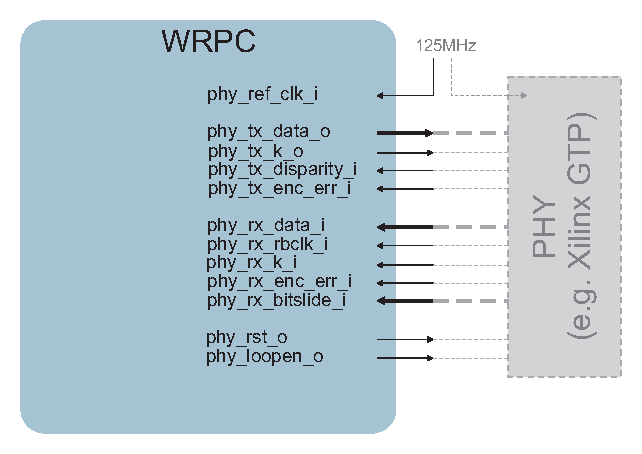
\includegraphics[width=.7\textwidth]{fig/wrpc_phyif.pdf}
    \caption{PHY interface of WRPC}
  \end{center}
\end{figure}

The interface connects WRPC with the Ethernet PHY layer IP-core. The interface is
generic, but currently two Gigabit Ethernet PHYs are tested and supported: Xilinx
8-bit GTP and 16-bit GTX SerDes. The signals' naming convention is the same as
in the GTP/GTX component definition.\\

{\bf Important !} If a WRPC user wants to use one of the supported PHYs (GTP,
GTX), they have to be taken from the White Rabbit HDL package instead of generating
them with the Xilinx Coregen tool. That is because WR developers have attached
additional logic to Xilinx GTP/GTX to improve its determinism.\\
